\chapter{Ergebnisse}
%Sandra
\Autor{Sandra Schröder}
\begin{itemize}
	\item Vergleich der Algorithmen
	\item Anhand der Kriterien: QUELLE!!!
	\begin{itemize}
		\item Erhaltung der Topologie
		\item Pixelkonnektivität
		\item Zentriert
		\item 1 Pixel breit
		\item Robustheit
	\end{itemize}
	\item Vergleich anhand von Screenshots
	\item Echtzeitfähigkeit -> Messungen machen -> Vergleich
	\item Verbesserung des Skeletts (Distanztransformation) mit Breitensuche um Pixelkonnektivität zu erreichen -> Weitere Verbesserungen? -> Ohne Features sondern anhand der weißen Pixel
	\item Anwendung: Vergleich von Posen -> Features bestimmen. Vllt sowas wie "Spannweite" der Pose in x und in y Richtung (Abstand des "linkesten" zum "rechtesten" Pixel). 
\end{itemize}
\section{Vergleich der Algorithmen}
\section{Echtzeitfähigkeit}
\section{Verbesserung der Skelettqualität}
Das Skelett, welches mit der Methode der Distanztransformation bestimmt wurde, weißt Lücken zwischen den Skelettteilen auf. Die Ursache ist der Gradientenbetrag, der für die Extraktion der Skelettlinie berechnet wurde, sowie die Segmentierung des Bildes. 
\begin{figure}
\centering
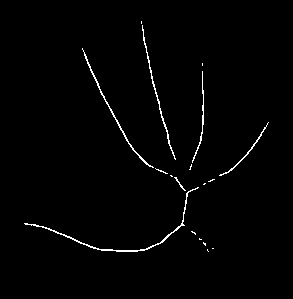
\includegraphics[width=0.4\linewidth]{./fig/hand-skelett}
\caption{Skelettierung mit der Distanztransformation. Das Skelett besitzt keine Pixelkonnektivität und weist große Lücken auf.}
\label{fig:hand-skelett}
\end{figure}
\subsection{Berechnung von Features auf dem Skelett}
\subsection{Breitensuche}
\subsection{Tiefensuche}